\documentclass{article}
\usepackage{amsmath, amssymb, graphicx}

\begin{document}

\begin{equation*}
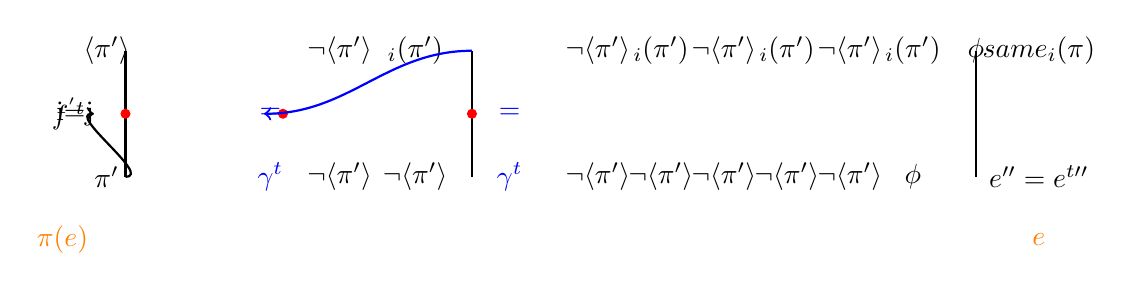
\begin{tikzpicture}[scale=0.8]
    \draw[thick] (-4,-1) -- (-4,1);
    \node at (-4.3, 1) {$\langle\pi'\rangle$};
    \node at (-4.3, -1) {$\pi'$};
    
    \draw[->, thick] (-4,-1) to [out=0, in=180] (-4.5,0);
    \filldraw[red] (-4,0) circle (2pt);
    \node at (-4.9, 0) {$f^{'t}$};
    
    \node at (-5,-2) {\textcolor{orange}{$\pi(e)$}};
    
    \draw[thick] (1.5,-1) -- (1.5,1);
    \node at (-0.6, 1) {$\neg\langle\pi'\rangle$};
    \node at (0.6, 1) {$\same_{i}(\pi')$};
    \node at (-0.6, -1) {$\neg\langle\pi'\rangle$};
    \node at (0.6, -1) {$\neg\langle\pi'\rangle$};
    
    \filldraw[red] (-1.5,0) circle (2pt);
    \node at (-1.7, 0) {\textcolor{blue}{$=$}};
    \node at (-1.7, -1) {\textcolor{blue}{$\gamma^{t}$}};
    
    \draw[->, blue, thick] (1.5,1) to [out=-180, in=0] (-1.8,0);
    \filldraw[red] (1.5,0) circle (2pt);
    \node at (2.1, 0) {\textcolor{blue}{$=$}};
    \node at (2.1, -1) {\textcolor{blue}{$\gamma^{t}$}};
    
    \node at (3.5, 1) {$\neg\langle\pi'\rangle$};
    \node at (4.5, 1) {$\same_{i}(\pi')$};
    \node at (5.5, 1) {$\neg\langle\pi'\rangle$};
    \node at (6.5, 1) {$\same_{i}(\pi')$};
    \node at (7.5, 1) {$\neg\langle\pi'\rangle$};
    \node at (8.5, 1) {$\same_{i}(\pi')$};
    \node at (9.5, 1) {$\phi$};
    
    \node at (3.5, -1) {$\neg\langle\pi'\rangle$};
    \node at (4.5, -1) {$\neg\langle\pi'\rangle$};
    \node at (5.5, -1) {$\neg\langle\pi'\rangle$};
    \node at (6.5, -1) {$\neg\langle\pi'\rangle$};
    \node at (7.5, -1) {$\neg\langle\pi'\rangle$};
    \node at (8.5, -1) {$\phi$};
    
    \draw[thick] (9.5,-1) -- (9.5,1);
    \node at (10.5, 1) {$same_{i}(\pi)$};
    \node at (10.5, -1) {$e'' = e^{t\prime\prime}$};
    \node at (10.5, -2) {\textcolor{orange}{$e$}};
    
    \node at (-4.8, 0) {i=j};
\end{tikzpicture}
\end{equation*}

\textit{Case $\pi=\prevon{i}{\varphi}\cdot\pi'$ and $t,e'' \models \phi$.}

\end{document}